\newpage
\section[\textsc{fubini's theorem}]{FUBINI'S THEOREM}\index{Fubini's Theorem}
The problem of calculating integrals is solved, in some sense,
by Theorem 3-10, which reduces the computation of integrals over a closed 
rectangle in $\F{R}^n, n > 1$, to the computation of integrals over closed intervals in $\F{R}$.
Of sufficient importance to deserve a special designation, this theorem is usually
referred to as Fubini's theorem, although it is more or less a special case of a 
theorem proved by Fubini long after Theorem 3-10 was known.

\begin{figure}[htb]
    \centering
    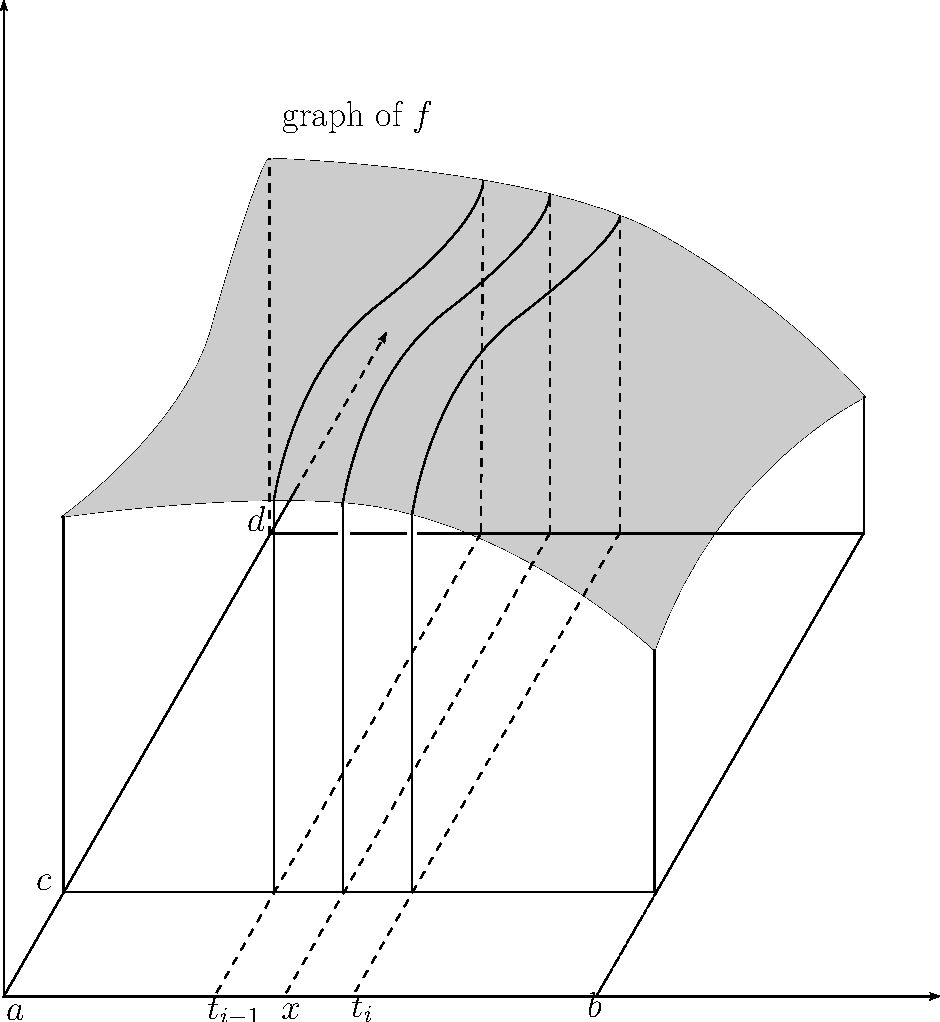
\includegraphics[width=.7\linewidth]{./pics/Fig3-2.pdf}
    \caption{}
    \label{Fig 3-2}
\end{figure}

The idea behind the theorem is best illustrated (Figure \ref{Fig 3-2})
for a positive continuous function  $f\colon{}[a,b]\times [c, d]\to \F{R}$. Let $t_0, \cdots, t_n$ 
be a partition of $[a, b]$ and divided $[a, b]\times [c, d]$ into $n$ strips by means of the 
lines segments $\{t_i\}\times [c, d]$. If $g_x$ is defined by $g_x(y) = f(x, y)$, then the area 
of the region under the graph of $f$ and above $\{x\}\times [c, d]$ is 
\begin{align*}
  \int_{c }^{d}{g_x} = \int_c^df(x, y)\;\dd y
\end{align*}

The volume of the region under the graph of $f$ and above $[t_{i-1},t_i] \times [c,d]$ 
is therefore approximately equal to $(t_i-t_{i-1})\cdot \int_c^d f(x,y)\;\dd y$, for any $x\in [t_{i-1}, t_i]$.
Thus 
\begin{align*}
  \int_{[a,b]\times [c, d]} f  = \sum_{i=1}^{n}{\int_{[t_{i-1}, t_i]\times [c, d] }f }
\end{align*}

is approximately $\sum_{i=1}^{n }{(t_i-t_{i-1}) \cdot \int_c^d f(x_i,y)\;\dd y} $, with $x_i$ in 
$[t_{i-1},t_i]$. On the other hand, sums similar to these appear in the definition of 
$\int_a^b\left(\int_c^d f(x, y)\;\dd y\right)\;\dd x$. Thus, if $h$ is defined by 
$h(x) = \int_c^d g_x = \int_c^d f(x, y)\;\dd y$, it is reasonable to hope that $h$ is 
intergrable and that 
\begin{align*}
    \int_{[a,b]\times [c, d]} f  
    = \int_a^b h
    = \int_a^b\left(\int_c^d f(x, y)\;\dd y\right)\;\dd x
\end{align*}

This will indeed turn out to be true when $f$ is continuous, but in the general case difficulties arise.
Suppose, for example, that the set of discontinuities of $f$ is $\{x_0 \} \times [c,d]$ for some
$x_0 \in [a,b]$. Then $f$ is integrable on $[a,b] \times [c,d]$ but $h(x_0) =\int_c^d f(x_0,y)\;\dd y$ 
may not even be defined. The statement of Fubini's theorem therefore looks a little strange, and will be
followed by remarks about various special cases where simpler statements are possible.

We will need one bit of terminology. If $f\colon{} A\to  \F{R}$ is a
bounded function on a closed rectangle, then, whether or not
$f$ is integrable, the least upper bound of all lower sums, and
the greatest lower bound of all upper sums, both exist.
They are called the lower\index{Integral!lower}\index{Lower integral} and upper\index{Integral!upper}\index{Upper integral} integrals of $f$ on $A$, and
denoted 
\begin{align*}
  \mathbf{L} \int_A f \text{\hspace*{3em} and \hspace*{3em}} \mathbf U\int_A f
\end{align*}
respectively. 

\begin{theorem}[Fubini's Theorem]
    Let $A\subset \F{R}^n$ and $B\subset \F{R}^m$ be closed rectangles, and 
    let $f\colon{} A\times B\to \F{R}$ be a integrable. Foe $x\in A$ let $g_x:B\to \F{R}$ be defined 
    by $g_x(y)=f(x, y)$ and let 
    \begin{align*}
        & \C{L}(x) = \mathbf{L}\int_B g_x = \mathbf{L}\int_B f(x, y)\;\dd y, \\
        & \C{U}(x) = \mathbf{U}\int_B g_x = \mathbf{U}\int_B f(x, y)\;\dd y.
    \end{align*}
    Then $\C{L}$ and $\C{U}$ are integrable on $A$ and 
    \begin{align*}
        & \int_{A\times B} f = \int_A \C{L} = \int_A \left(\mathbf{L}\int_B f(x, y)\;\dd y\right)\;\dd x \\
        & \int_{A\times B} f = \int_A \C{U} = \int_A \left(\mathbf{U}\int_B f(x, y)\;\dd y\right)\;\dd x
    \end{align*}
\end{theorem}
\noindent(The integrals on the right side are called \textbf{iterated integrals}\index{Iterated integral}\index{Integral!iterated} for $f$.)

\begin{proof}
    Let $P_A$ be a partition of $A$ and $P_B$ a partition of $B$.
    Together they give a partition $P$ of $A \times B$ for which any
    subrectangle $S$ is of the form $S_A \times S_B$, where $S_A$ is 
    a subrectangle of the partition $P_A$, and $S_B$ is a subrectangle of the
    partition $P_B$. Thus
    \begin{align*}
        L(f, P)
        & = \sum_{S }^{}{m_S(f)\cdot v(S)} \\
        & = \sum_{S_A, S_B}^{}{m_{S_A\times S_B}(f)\cdot v(S_A\times S_B)} \\
        & = \sum_{S_A}^{}{\left(\sum_{S_B}^{}{m_{S_A\times S_B}(f)\cdot v(S_B)}\right)\cdot v(S_A)} 
    \end{align*}

    Now, if $x\in S_A$, then clealy $m_{S_A\times S_B}(f) \le m_{S_b}(g_x)$. Consequently, for $x\in S_A$
    we have 
    \begin{align*}
        \sum_{S_B}m_{S_A\times S_B}(f)\cdot v(S_B)\leq\sum_{S_B}m_{S_B}(g_x)\cdot v(S_B)\leq\mathbf{L}\int_Bg_x=\C{L}(x)
    \end{align*}

    Therefore 
    \begin{align*}
        \sum_{S_A}\left(\sum_{S_B}m_{S_A\times S_B}(f)\cdot v(S_B)\right)\cdot v(S_A)\leq L(\mathcal{L},P_A)
    \end{align*}

    We thus obtain
    \begin{align*}
        L(f,P)\leq L(\mathcal{L},P_A)\leq U(\mathcal{L},P_A)\leq U(\mathcal{U},P_A)\leq U(f,P)
    \end{align*}

    where the proof of the last inequality is entirely analogous to the proof of the first.
    Since $f$ is integrable, $\sup \{L(f, p)\}=\inf\{U(f, P)\} = \int_{A\times B} f$. Hence 
    \begin{align*}
        \sup\{f, P\} \le L(\mathcal{L},P_A)
        \le L(\mathcal{L},P_A)
        \le U(\mathcal{U},P_A)
        \le \sup\{U(f, P)\}
    \end{align*}
\end{proof}

\noindent\textbf{Remarks.} 
\begin{enumerate}[label={\textup{\arabic*.\,}}]
    \item A similar proof shows that
        \begin{align*}
            \int_{A\times B}f
            = \int_{B}\left(\mathbf{L}\int_{A}f(x,y)\dd x\right)\dd y
            = \int_{B}\left(\mathbf{U}\int_{A}f(x,y)\dd x\right)\dd y.
        \end{align*}
        These integrals are called iterated integrals\index{Integral!iterated}\index{Iterated integral} for $f$ in the reverse
        order from those of the theorem. As several problems show,
        the possibility of interchanging the orders of iterated integrals
        has many consequences.
    \item In practice it is often the case that each $g_x$ is integrable, so that
        $\int_{A\times B} f = \int_A\left(\int_B f(x, y)\;\dd y\right)\dd x$. This certainly
        occurs if $f$ is continuous.
    \item The worst irregularity commonly encountered is that $g_x$
        is not integrable for a finite number of $x\in A$. In this case 
        $\C{L}(x) =\int_B f(x, y) \;\dd y$ for all but these finitely many $x$. Since 
        $\int_A \C{{L}}$ remains unchanged if $\C{L}$ is refined at a finite number of 
        points, we can still write $\int_{A\times B} f = \int_A \left(\int_B f(x, y)\;\dd y\right)\;\dd x$,
        provided that $\int_B f(x, y)\; \dd y$ is defined arbitarily, say as 0, when it dose not exist.
    \item There are cases when this will not work and Theorem 3-10
    must be used as stated. Let $f\colon{}[0,1]\times [0,1]\to\F{R}$ be defined by 
    \begin{align*}
        f(x,y)
        = \left\{\begin{aligned}
            & 1 && \text{if $x$ is irrational}, \\
            & 1 && \text{if $x$ is rational and $y$ is irrational}, \\
            & 1-1/q && \text{if $x=p/q$ in lowest terms and $y$ is rational}.
        \end{aligned}\right.
    \end{align*}
    Then $f$  is integrable and $\int_{[0,1]\times [0,1] f} = 1$. Now $\int_0^1f(x, y)\;\dd y=1$ if 
    $x$ is irrational, and does not exist if $x$ is rational. Therefore $h$ is not integrable 
    if $h(x) = \int_0^1 f(x, y)\;\dd y$ is set equal to 0 when the integral dose not exist. 
    \item If $C\subset A\times B$, Fubini's theorem can be used to evaluate $\int_Cf$, since 
        this is by definition $\int_{A\times B}f\cdot \chi_Cf$. Suppose, for example, that 
        \begin{align*}
            \int_C f 
            = \int_{-1}^1 \left(\int_{-1}^1 f(x, y)\cdot \chi_C(x,y)\;\dd y\right)\;\dd x.
        \end{align*}
        Now 
        \begin{align*}
            \chi_C(x, y)
            = \left\{\begin{aligned}
                & 1 && \text{ if $y>\sqrt{1-x^1}$ or $y<-\sqrt{1-x^2}$},\\
                & 0 && \text{ otherwise}.
            \end{aligned}\right.
        \end{align*}
        Therefore 
        \begin{align*}
            \int_{-1}^1 f(x,y)\cdot \chi_C(x,y)\;\dd y
            = \int_{-1}^{-\sqrt{1-x^2}} f(x, y)\;\dd y 
                + \int_{\sqrt{1-x^2}}^{1} f(x, y)\;\dd y.
        \end{align*} 

        In general, if $C\subset A\times B$, the main diffculty in deriving expressions for 
        $\int_C f$ will be determining  $C\cap (\{x\}\times B)$ for $x\in A$. If $C\cap (A\times \{y\})$
        for $y\in B$ is easier to determine, one should use the iterated integral
        \begin{align*}
            \int_C f 
            = \int_B\left(\int_A f(x, y)\cdot \chi_C(x, y)\,\dd x \right)\dd y.
        \end{align*}
\end{enumerate}

\begin{problems}
    \problem{
        Let $C\subset A\times B$ be a set of content 0. Let  $A'\subset A$ be the set of all 
        $x\in A$ such that $\{y\in B:(x, y)\in C\}$ is not of content 0. Show that $A'$ is a set 
        of measure 0. \textit{Hint:} $\chi_C$ is integrable and $\int_{A\times B}\chi_C = \int_A\C{U} 
        =\int_A\C{L}$, so $\int_A \C{U}-\C{L} = 0$.
    }
    \problem{
        Let $C \subset [0,1] \times [0,1]$ be the union of all $\{p/q\} \times [0, 1/q]$, where
        $p/q$ is a rational number in $[0,1]$ written in lowest terms. Use $C$ to show that 
        the word "measure" in Problem 3-23 cannot be replaced by ``content.''
    }
    \problem{
        Use induction on n to show that $[a_1, b_1]\times \cdots \times [a_n, b_n]$ is not a  
        set of measure 0. (or content 0) if $a_i<b_i$ for each $i$.
    }
    \problem{
        Let $f\colon{}[a,b]\to \F{R}$ be integrable and non-intergrable and let $A_f = \{
        (x, y):a\le x\le b\text{ and } 0\le y\le f(x)\}$. Show that $A_f$ is Jordan-measurable
        and has area $\int_a^b f$.
    }
    \problem{
        If $f\colon{}[a, b]\times [a, b]\to \F{R}$ is continuous, show that 
        \begin{align*}
            \int_a^b\int_a^y f(x, y)\;\dd x\dd y = 
            \int_a^b\int_x^b f(x, y)\;\dd y\dd x.
        \end{align*}
        \textit{Hint:} Compute $\int_Cf$ in to different ways for a suitable set 
        $C\subset [a, b]\times [a,b]$.
    }
    \problem[*]{
        Use Fubini's theorem to give ann easy proof that $\R{D}_{1,2}f = \R{D}_{2,1}f$
        if these are continuous. \textit{Hint:} If $\R{D}_{1,2}f-\R{D}_{2,1}f>0$, there is 
        a rectangle $A$ containing a such that $\R{D}_{1,2}f-\R{D}_{2,1}f>0$ on $A$.
    }
    \problem{
        Use Fubini's theorem to derive an expression for the volume of
        a set of $\F{R}^3$ obtained by revolving a Jordan-measurable set in the
        $yz$-plane about the $z$-axis.
    }
    \problem{
        Let C be the set in Problem 1-17. Show that
        \begin{align*}
            \int_{[0,1]} \left(\int_{[0,1]}\chi_C(x,y)\;\dd x\right)\;\dd y 
            = \int_{[0,1]}\left(\int_{[0,1]}\chi_C(y,x)\;\dd y\right)\;\dd x
            = 0
        \end{align*}
        but that $\int_{[0,1]\times [0,1]} \chi_C$ dose not exist.
    }
    \problem{
        If $A=[a_1, b_1]\times \cdots \times [a_n,b_n]$ and $f\colon{}A\to \F{R}$ is continuous, 
        define $f\colon{}A\to \F{R}$ by 
        \begin{align*}
            F(x) = \int_{[a_1, x^1]\times \cdots \times [a_n, x^n]} f
        \end{align*}
        What is $\R{D}_iF(x)$, for $x$ in the interior of $A$?
    }
    \problem[*]{
        Let $f\colon{}[a, b]\times [c,d]\to \F{R}$ be continuous and suppose $\R{D}_2f$ is continuous.
        Define $F(y)=\int_a^bf(x, y)\;\dd x$. Prove \textit{Leibnitz's rule}\index{Leibnitz's Rule}: 
        $F'(y) = \int_a^b\R{D}_2f(x,y)\;\dd x$. \textit{Hint:} $F(y)=\int_a^bf(x,y)\;\dd x
        =\int_a^b\left(\int_c^y\R{D}_2f(x, y)\;\dd y\right) + f(x, c)\;\dd x$.(The proof will show that 
        continuity of $\R{D}_2f$ may be replaced by considerably weaker hypothese.)
    }
    \problem{
        If $f\colon{}[a,b]\times [c,d]\to \F{R}$ is continuous and $\R{D}_2f$ is continuous, define 
        $F(x,y) = \int_a^xf(t, y)\;\dd t$.
        \begin{enumerate}[label=(\alph*)]
            \item Find $\R{D}_1F$ and $\R{D}_2F$.
            \item If $G(x) = \int_a^{g(x) f(t, x)\;\dd t}$, find $G'(x)$.
        \end{enumerate}
    }
    \problem[*]{
        Let $g_1,g_2:\F{R}^2\to \F{R}$ be continuously differentiable and suppose
        $\R{D}_1g_2 = \R{D}_2g_1$. As in Problem 2-21, let 
        \begin{align*}
            f(x, y) = \int_0^xg_1(t, 0)\;\dd t + \int_0^yg_2(x, t)\;\dd t
        \end{align*}
        Show that $\R{D}_1f(x, y) = g_1(x, y)$.
    }
    \problem[*]{
        \begin{enumerate}[label=(\alph*)]
        \item Let $g\colon{}\F{R}^n\to\F{R}^n$ be linear transformation of one of the following types:
            \begin{align*}
                & \left\{\begin{aligned}
                    & g(e_i) = e_i, i\neq j \\
                    & g(e_j) = ae_j
                \end{aligned}\right.
                && \left\{\begin{aligned}
                    & g(e_i) = e_i, i\neq j \\
                    & g(e_j) = e_j + e_k \\
                \end{aligned}\right.\\[2em]
                & \left\{\begin{aligned}
                    & g(e_k) = e_k, k\neq i,j \\
                    & g(e_i) = e_j\\
                    & g(e_j) = e_i 
                \end{aligned}\right.
            \end{align*}
            If $U$ is a rectangle, show that the volume of $g(U)$ is $|\det g|\cdot v(U)$.
        \item Prove that $|\det g|\cdot v(U)$ is the volume of $g(U)$ for any linear transformation 
            $g\colon{}\F{R}^n\to\F{R}^n$. \textit{Hint:} If $\det g\neq 0$, then $g$ is the 
            composition of linear transformations of the types considering in (a).
    \end{enumerate}
    }
    \problem{
        (Cavalieri's principle)\index{Cavalieri's principle} Let $A$ and $B$ be Jordan-measurable sets in $\F{R}^3$.
        Let $A_c = \{(x,y):(x,y,c)\in A\}$ and define $B_c$ similarly. Suppose each $A_c$ and 
        $B_c$ are Jordan-meausrable and have the same area. Show that $A$ and $B$ have the same volume.
    }
\end{problems}